% kapitel6.tex
\externaldocument{02_grundlagen.tex}
\chapter{Ergebnisse und Diskussion}
\label{chapter:ergebnisse}

\section{Versuchsergebnisse}
\label{section:versuchsergebnisse}

Im folgenden Kapitel werden zunächst die Ergebnisse der Evaluation dargestellt und im Anschluss folgt die Diskussion der gewonnenen Ergebnisse. 

\subsection{Parcoursdurchführung}
Mittels der Zeitmessung während der Parcoursbewältigungsaufgabe sollte die Machbarkeit der bereitgestellten Steuerungsmethoden (diskret und kontinuierlich) demonstriert und abgeschätzt werden. 
\acs{tab} \ref{tab:parcourzeit} und die \acs{abb} \ref{fig:parcourzeit} zeigen die ermittelten Durchführungszeiten der Testpersonen der Testparcoursaufgabe.

\begin{figure}[ht]
\begin{center}
\fbox{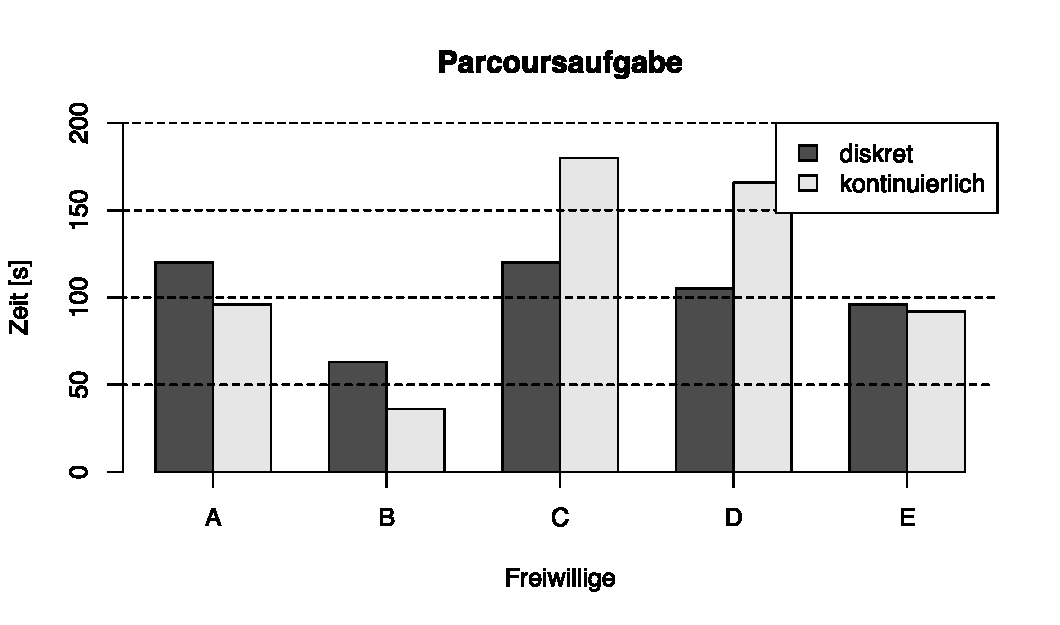
\includegraphics[width=0.7\textwidth]{bilder/ergebnisse/parcours680x400.pdf}}
\end{center}
\caption{Zeit der Parcoursbewältigung der fünf Testpersonen (\enquote{A},\enquote{B},\enquote{C},\enquote{D},\enquote{E}) in Abhängigkeit der Steuerungsmethode (Zeit in Sekunden).}
\label{fig:parcourzeit}
\end{figure}


\begin{table}[h]
\centering
\begin{tabular}{crrrrr}
  \hline
 & A & B & C & D & E \\ 
  \hline
diskret & 120 &  63 & 120 & 105 &  96 \\ 
  kontinuierlich &  96 &  36 & 180 & 166 &  92 \\ 
   \hline
\end{tabular}
\caption{Zeit der Parcoursbewältigung der fünf Testpersonen (\enquote{A},\enquote{B},\enquote{C},\enquote{D},\enquote{E}) in Abhängigkeit der Steuerungsmethode (\enquote{diskret}, \enquote{kontinuierlich}) (Angaben in Sekunden).} 
\label{tab:parcourzeit}
\end{table} 

Wie in \acs{abb}~\ref{fig:parcourzeit} zu erkennen ist, konnte jede der Testpersonen die gestellte Parcoursaufgabe mittels der beschriebenen Steuermethoden bewältigen. Testperson \enquote{B} zeigte im Vergleich für beide Steuermethoden die geringste Durchführungszeit und Testperson \enquote{C} benötigte für die kontinuierliche Steuermethode am längsten. Die minimale Durchführungszeit konnte mit der kontinuierlichen Methode erzielt werden (36 Sekunden). Die maximale Durchführungszeit wurde ebenfalls mit der kontinuierlichen Steuerungsmethode erzielt (180 Sekunden), \vgl~\acs{tab}~\ref{tab:parcourstat}. Die durchschnittliche Durchführungszeit lag bei der diskreten Steuermethode bei 100.8 Sekunden und bei der kontinuierlichen bei 114 Sekunden, \vgl~\acs{tab}~\ref{tab:parcourstat}. Bei drei der fünf Testpersonen war die Durchführungszeit der kontinuierlichen Steuermethode im Vergleich zur diskreten Steuerungsmethode schneller. 

\begin{table}[h]
\centering
\begin{tabular}{lcc}
  \hline
 &    diskret & kontinuierlich \\ 
  \hline
Min.   :&  63   & 36   \\ 
 Median : & 105  & 96   \\ 
 Mean   : & 100.8   & 114   \\  
 Max.   : & 120  &    180   \\ 
   \hline
\end{tabular}
\caption{Tabelle des Minimum (Min), Maximum (Max), Median (Median), arithmetischer Durchschnitt (Mean) in Abhängigkeit der Steuermethode.} 
\label{tab:parcourstat}
\end{table}

\subsection{Unerwünschte Ausführungen}
Bei der Benutzung des Prototyps kam es zu unbeabsichtigten Ausführungen. \acl{abb}~\ref{fig:ausführungen} zeigt deren Häufungen im Verhältnis zu den möglichen Aktionen.
\begin{figure}[ht]
\begin{minipage}[t]{\linewidth} 
\centering
\fbox{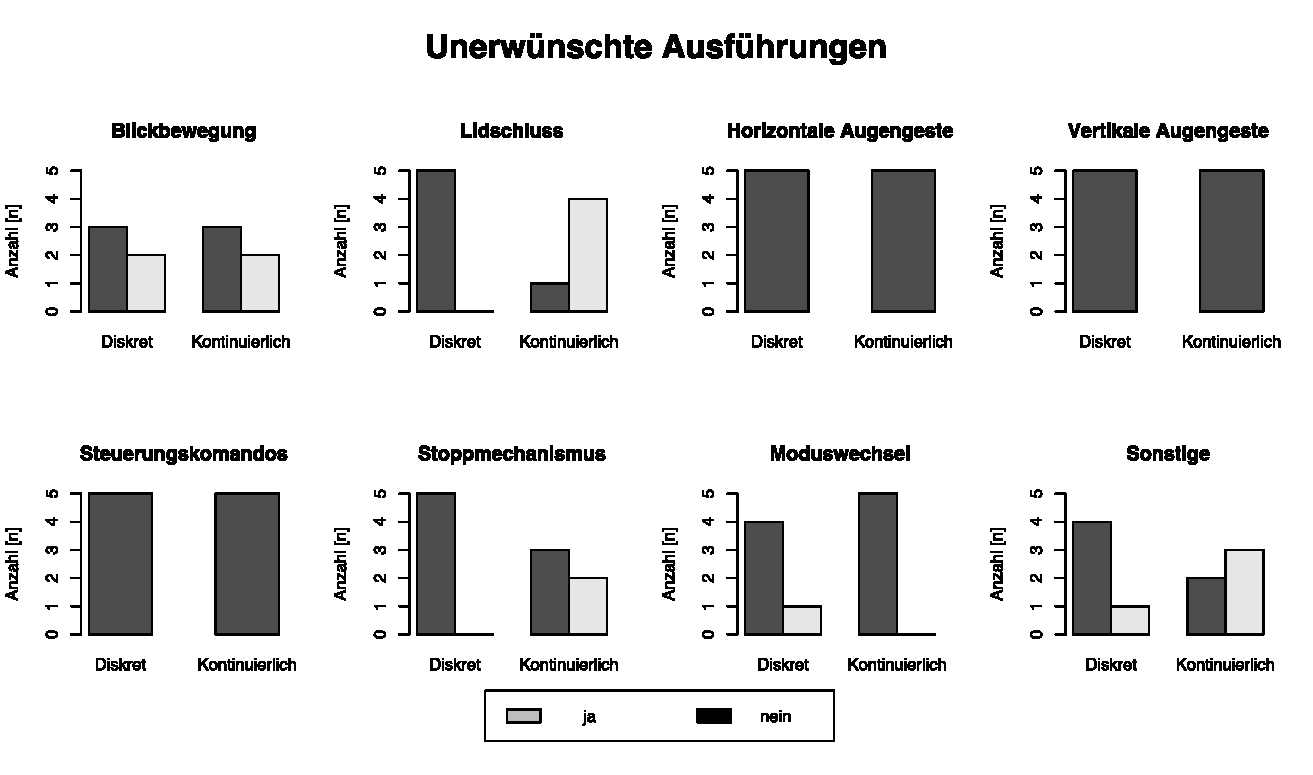
\includegraphics[width=0.7\textwidth]{bilder/ergebnisse/ausfuehrungen880x4402.pdf}}
\caption{Unerwünschte Ausführungen während des gesamten Durchführungszeitraums.}
\label{fig:ausführungen}
  \end{minipage}% 
\end{figure}

Die Auswertung der Mehrfachantworten zeigt, dass keine der Personen unerwünschte Ausführungen bei der horizontalen- und vertikalen Augengeste oder den Steuerkommandos hatte. Dies gilt sowohl für die diskrete, als auch für die kontinuierliche Steuermethode. Bei vier der fünf Benutzer war der Lidschluss während der kontinuierlichen Steuermethode in Bezug auf unerwünschte Ausführungen die problematischste Augengeste. Während der Ausführung der diskreten Steuermethode kam es zu keinen unerwünschten Ausführungen beim Lidschluss. Bei der Ausführung des kontinuierlichen Steuermodus traten bei zwei Personen während des Stoppmechanismus unerwünschte Ausführungen auf. Die Nutzung des kontinuierlichen Steuermodus verlief während des Stoppmechanismus bei allen Testpersonen störungsfrei. Die Blickbewegung führte sowohl während der Nutzung des kontinuierlichen, als auch des diskreten Steuermodells zu unerwünschten Ausführungen bei jeweils zwei Testpersonen. 
Die Möglichkeit einer zusätzlichen Angabe durch die Option \enquote{Sonstiges} wurde von zwei Personen genutzt.
Eine Testperson gab sowohl für die diskrete, als auch für die kontinuierliche Steuermethode an, dass unerwünschte Ausführungen während der Kopfbewegung auftraten. Eine Testperson hatte während der Nutzung der kontinuierlichen Steuermethode Probleme, weil das System \enquote{gelegentlich nicht mehr auf Augengesten} reagierte. 


\subsection{Ermüdung}
Mittels der vierstufigen Ratingskala wurde nach der Ausführung der Parcoursbewältigungsaufgabe abgeschätzt, als wie ermüdend die beiden angebotenen Steuermethoden empfunden wurden. \acl{abb}~\ref{fig:ermüdung} veranschaulicht die Angaben grafisch.
\begin{figure}[ht]
\begin{minipage}[b]{\linewidth} 
      \centering 
\fbox{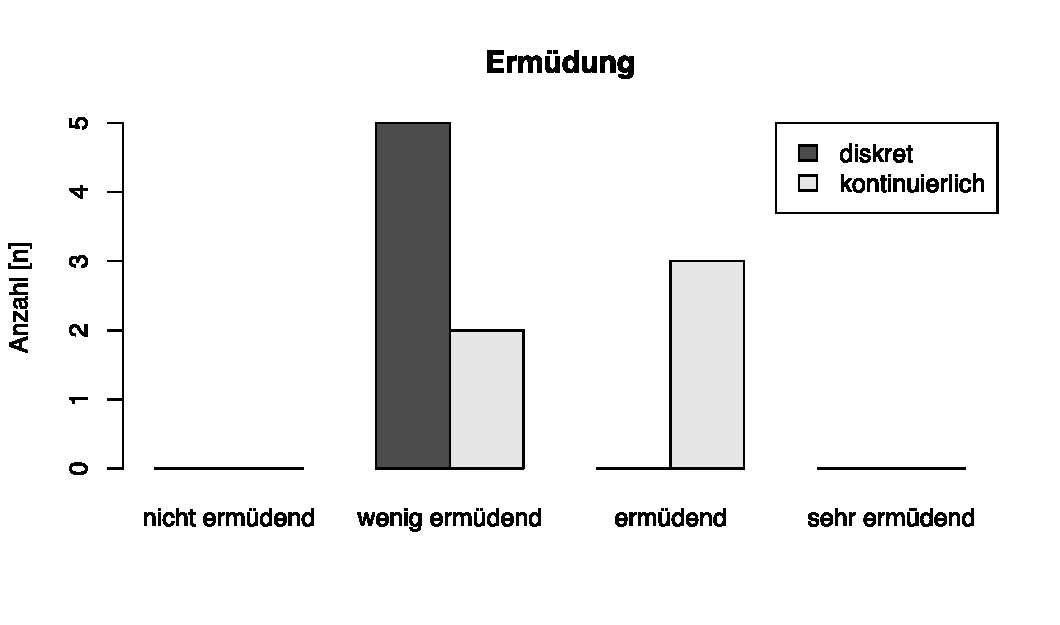
\includegraphics[width=0.7\textwidth]{bilder/ergebnisse/ermuedung680x400.pdf}}
\caption{Diagramm zur Bewertung der Ermüdung}
\label{fig:ermüdung}
   \end{minipage}% 
\end{figure}
\begin{comment}
\begin{figure}[ht]
   \begin{minipage}[b]{\linewidth} 
      \centering 
     %\includegraphics[scale=1]{bilder/grundlagen/als.pdf}
     % \includegraphics[width=1\textwidth]{bilder/grundlagen/1als.pdf}
     \fbox {\includegraphics[width=\textwidth, height=100mm]{bilder/grundlagen/Ermu_dung.pdf}}
   \end{minipage}% 
\caption{Diagramm zur Bewertung der Ermüdung}
\label{fig:ermüdung}
\end{figure} 
\end{comment}


Die \acl{abb}~\ref{fig:ermüdung} veranschaulicht, dass alle fünf Testpersonen die Steuerung mittels diskreter Steuermethode als \enquote{wenig ermüdend} eingestuft haben. Die kontinuierliche Steuermethode wurde lediglich von zwei Testpersonen als \enquote{wenig ermüdend} eingeschätzt, während drei weitere Personen sie als \enquote{ermüdend} empfanden. 

\subsection{Handling}
Neben den unerwarteten Ausführungen und der Ermüdung, wurde als drittes Merkmal mithilfe der vierstufigen Ratingskala abgeschätzt, wie einfach das Handling der beiden Steuerungsmethoden empfunden wurde. \acl{abb}~\ref{fig:handling} zeigt die Angaben der Testpersonen grafisch.
\begin{figure}[ht]
\begin{minipage}[t]{\linewidth} 
      \centering 
\fbox{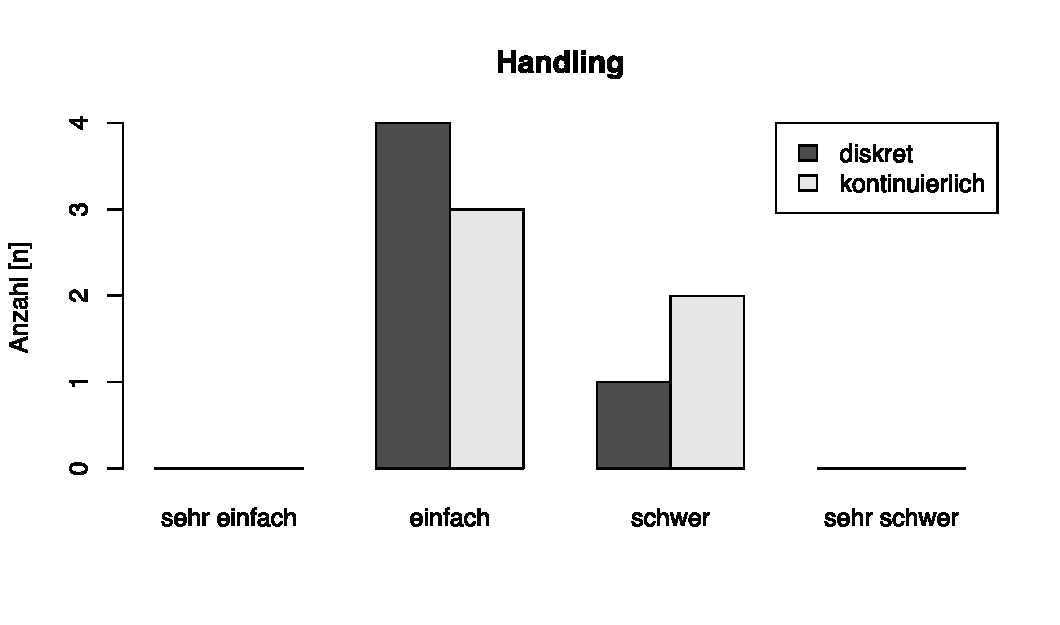
\includegraphics[width=0.7\textwidth]{bilder/ergebnisse/handling680x400.pdf}}
\caption{Diagramm zur Bewertung des Handlings.}
\label{fig:handling}
   \end{minipage}% 
\end{figure}

Wie in \acs{abb}~\ref{fig:handling} ersichtlich, empfanden vier der fünf Testpersonen die Steuerung mittels der diskreten Steuermethode als \enquote{einfach}, nur eine Person stufte sie als \enquote{schwer} ein. Die kontinuierliche Steuermethode wurde von drei Testpersonen als \enquote{einfach} eingeschätzt, zwei Personen empfanden sie als \enquote{schwer}. Keine der Testpersonen empfand das Handling der Steuerung als \enquote{sehr einfach} oder \enquote{sehr schwer}. Im Vergleich zur kontinuierlichen Steuermethode wurde die diskrete Steuermethode hierbei tendenziell einfacher wahrgenommen und evaluiert.

\subsection{Panikschalter}
Als weiteres Merkmal wurde mittels der \og vierstufigen Ratingskala abgeschätzt, wie einfach das Handling des Panikschalters der beiden Steuerungsmethoden empfunden wurde. \acl{abb}~\ref{fig:panikschalter} stellt die Angaben der Testpersonen grafisch dar. Hierbei machte eine der Testpersonen keine Angaben, weshalb nur bei (n=4) der Testpersonen eine Einschätzung möglich war. 
\begin{figure}[hbt]
\centering
\fbox{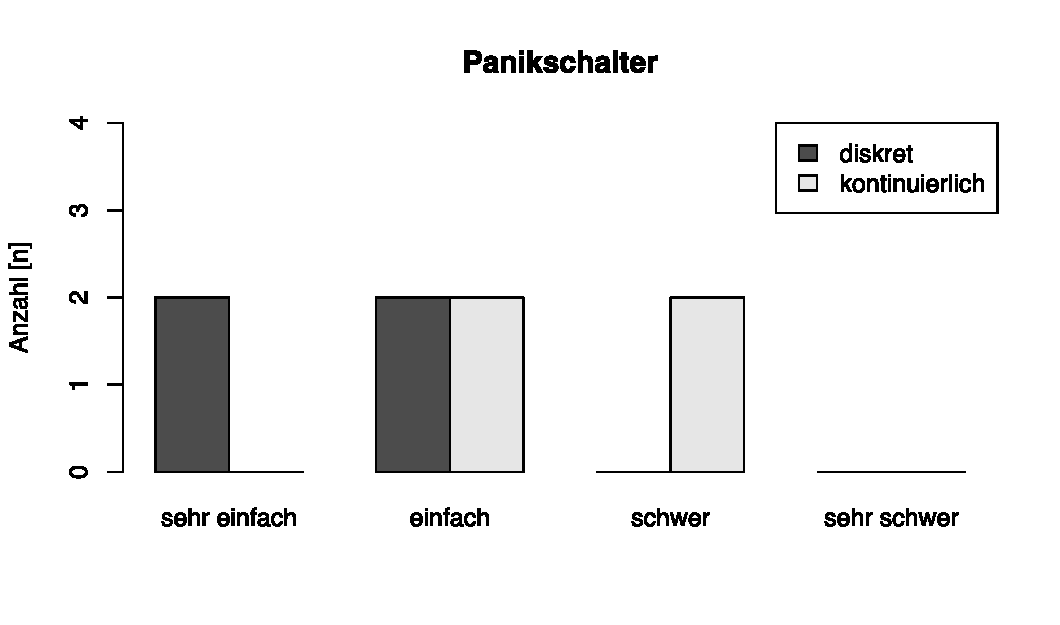
\includegraphics[width=0.7\textwidth]{bilder/ergebnisse/panikschalter680x400.pdf}}
\caption{Diagramm zur Bewertung des Panikschalters.}
\label{fig:panikschalter}
\end{figure}

Die \acl{abb}~\ref{fig:panikschalter} zeigt, dass zwei der vier Testpersonen das Handling des Panikschalters mittels der diskreten Steuermethode als \enquote{sehr einfach} und zwei Testpersonen dies als \enquote{einfach} einstuften. Im Fall der kontinuierlichen Steuermethode wurde von zwei Testpersonen die Einschätzung \bzgl des Panikschalters als \enquote{einfach} und von zwei weiteren Personen als \enquote{schwer} eingestuft. Keine der Testpersonen empfand das Handling des Panikschalters als \enquote{sehr schwer}. Der Panikschalter wurde während der Nutzung der diskreten Steuermethode,- (im Vergleich zur kontinuierlichen Steuermethode) als einfach wahrgenommen und evaluiert.

\subsection{Erweiterte Steuerungsoptionen}
Erweiterte Steuerungsoptionen wurden mittels Mehrfachantwort durch die Benutzer erfragt.
Die Auswertung zeigt, dass sich alle fünf Testpersonen eine Erweiterung der Steuerung um eine Kollisionsvermeidung wünschten. Keiner der fünf Beteiligten wünschte sich eine Augmentation der Steuerung um die Möglichkeit einer \enquote{Fahre an Ort (GOTO)}-Option oder einer \enquote{Folge einer Person (Follow)}-Option. Auch die zusätzliche Option einer Routenplanung wurde von keiner der Testpersonen gewünscht. 

Die Möglichkeit einer zusätzlichen Angabe durch die Option \enquote{Sonstiges} wurde von drei Personen genutzt.
Eine Testperson hielt die Steuerung mittels eines \enquote{Skalierungsfaktors} im Rahmen der kontinuierlichen Steuerung für wünschenswert. Eine weitere Testperson wünschte sich die Möglichkeit, die Kameraposition zu verändern, und eine Kamera, die den mobilen Roboter aus der Sicht einer dritten Person zeigt. Die dritte Testperson erachtete eine Anzeige zur Visualisierung des Abstandes zu Objekten in der unmittelbaren Umgebung des mobilen Roboters als wünschenswert.

\subsection{Gesamtbewertung}
Als Gesamtbeurteilung vergaben die Testpersonen Schulnoten auf einer Skala, die in \acs{abb}~\ref{fig:gesamtnoten} dargestellt ist.  
\begin{figure}[htb]
\begin{center}
\fbox{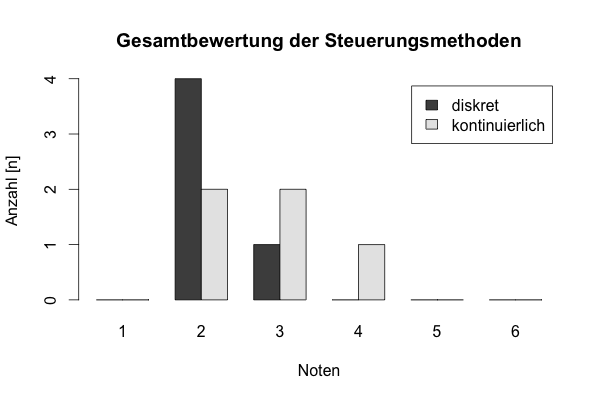
\includegraphics[width=0.7\textwidth]{bilder/ergebnisse/Gesamtbewertung.png}}
\end{center}
\caption{Gesamtbewertung in Schulnoten.}
\label{fig:gesamtnoten}
\end{figure}

Vier der fünf Testpersonen bewerteten die diskrete Steuerungsmethode mit \enquote{gut = 2}, einer der Benutzer mit \enquote{befriedigend = 3}. Die kontinuierliche Steuerungsmethode wurde von zwei der fünf Testpersonen mit \enquote{gut = 2} und von zwei weiteren mit \enquote{befriedigend = 3} bewertet. Die fünfte Testperson vergab hierfür die Note \enquote{ausreichend = 4}. Für beide Testmethoden wurden weder die Noten \enquote{sehr gut = 1}, noch die Bewertungen \enquote{mangelhaft = 5} oder \enquote{ungenügend = 6} vergebenen, siehe \acs{abb}~\ref{fig:gesamtnoten}.

\section{Diskussion}
\label{section:Diskusion}
Mobile~\aclp{tps} mittels definierter Augengesten zu steuern, ist -wie im Abschnitt~\ref{chapter:grundlagen} gezeigt wurde- eine anspruchsvolle Aufgabe. Das Ziel der vorliegenden Arbeit ist es, zwei unterschiedliche Lösungsstrategien für die Steuerung eines Telepräsenzrobotersystems in einem Softwareprototypen zu realisieren und diese \bzgl der Machbarkeit, der Präzision, der Handhabung, der Ermüdung und in Bezug auf die Nutzung eines Panikschalter zu vergleichen.
Es folgt die Diskussion der in Kapitel~\ref{section:versuchsergebnisse} beschriebenen Ergebnisse. Zunächst werden die beiden Steuerungsmethoden diskutiert und im Anschluss folgt die Diskussion der Testparameter und der Testpersonen.


\subsection{Diskussion der Steuerungsmodelle}
%Mittels der Zeitmessung während der Parcourbewältigungsaufgabe konnte die Machbarkeit der bereitgestellten Steuerungsmethoden (diskret, kontinuierlich) demonstriert werden. Die Evaluationsergebnisse zeigen, dass die Umsetzung einer Steuerung eines mobilen Roboters mithilfe eines Eyetrackers erfolgreich umgesetzt werden konnte. 

Die \og Evaluationsergebnisse demonstrieren, dass alle beteiligten Testpersonen die Parcoursaufgabe bewältigen konnten. Damit ist es grundsätzlich möglich, ein mobiles Robotersystem durch einen \enquote{einfachen}~Parcours nur mittels der Augen zielgerichtet zu manövrieren. Die bereitgestellten Steuerungsmethoden (diskret, kontinuierlich) wurden hierbei so konzipiert, dass eine \enquote{einfache} Basissteuerung durch das \textit{diskrete}~Steuermodell und eine \enquote{anspruchsvollere}~Steuerungsform durch die \textit{kontinuierliche} Steuermethode miteinander verglichen werden konnten. 
Wie die Gesamtbewertung zeigt, wurde die diskrete Steuermethode seitens der Testpersonen im Vergleich zur kontinuierlichen Steuerung tendenziell besser bewertet. Hierfür sprechen mehrere Gründe: Wie in \acs{abb}~\ref{fig:ausführungen} gezeigt, sind zum einen die unerwünschten Ausführungen während der Nutzung der diskreten Steuermethode insgesamt seltener aufgetreten. Dies kann seitens der Testpersonen positiv aufgefasst worden sein. Ferner kann das Fehlen der unerwünschten Ausführungen zu einem einfacheren Ablauf während der Steuerung geführt und die Bewertung beeinflusst haben. Der Faktor der \textit{Ermüdung} spielt für das Empfinden und damit die Bewertung ebenfalls eine wichtige Rolle. Die diskrete Steuerungsmethode wurde im Vergleich zur kontinuierlichen  als \enquote{weniger ermüdend} wahrgenommen. Auch in der Handhabung (Handling) wurde die diskrete Steuermethode tendenziell als einfacher empfunden. Darüber hinaus ist in Bezug auf die Nutzbarkeit das Stoppen des mobilen Roboters wichtig. Ein fehlendes Ansprechen bei einem Stoppkommando kann in kritischen Situationen unter Umständen zu schwerwiegenden Komplikationen führen. Daher ist der Stoppmechanismus für die Steuerung entscheidend.

Bezüglich der gemessenen Durchführungszeiten variierten die Ergebnisse teilweise deutlich zwischen den verschiedenen Testpersonen, siehe \acs{abb}~\ref{fig:parcourzeit}. Ein Hauptgrund dafür lag vermutlich in einem unterschiedlichen Erfahrungsniveau der Testpersonen in Bezug auf die Nutzung von Eyetracking-Systemen. Es zeigte sich jedoch, dass selbst gänzlich unerfahrenen Testpersonen der Zugang zur Nutzung eines Eyetracking-Systems und somit zur Steuerung des mobilen Roboters nach kurzer Zeit möglich war. Personen mit Bewegungseinschränkungen könnten von diesem Aspekt der relativ steilen Lernkurve profitieren. Alternative Mensch-Computer-Schnittstellen, wie beispielsweise abgeleitete Hirnstrommessungen mittels Elektroenzephalogramm (EEG), die zur Steuerung benutzt werden können, zeigen hier eine längere Eingewöhnungszeit, \vgl~\cite{Tonin2011}. Ferner sind diese Verfahren nach individueller Anpassung nicht problemlos auf andere Anwender übertragbar und müssen kalibriert werden. Die notwendige Kalibrierung der Eyetracking-Systeme ist bei vorhandener Augenmotorik relativ leicht umsetzbar. 
%Insgesamt ist es im Hinblick auf die \og Ergebnisse als ein gutes Ergebnisse zu werten, dass alle Testpersonen 

\subsection{Diskussion der Testmerkmale}
Die Arbeitsfragen bezüglich der Machbarkeit, der Präzision, des Handlings und die Fragen, wie ermüdend diese Art der Steuerung ist und ob Unterschiede zwischen einer diskreten und kontinuierlichen Steuerungsform vorhanden sind, wurden mittels eines eigens entworfenen Fragebogens beantwortet. Hierbei wurde versucht, die Machbarkeit und die Präzision durch die Quantifizierung der Durchführungszeit einer Parcoursaufgabe zu messen. Damit sollte eine einfache Vergleichbarkeit der beiden Steuerungsmethoden erreicht werden. Ferner wurde eine qualitative Bewertung des Handlings, der Ermüdung und des Panikschalters untersucht. Um die Motivation der Teilnehmer zu erhöhen, wurde der Fragebogen \bzgl der Ausfüllzeit kurz gehalten. 

\subsection{Diskussion der Testpersonen}
Bei der Durchführung der Evaluation und der Benutzung des Prototyps wurden fünf gesunde Testpersonen befragt und \bzgl der Parcoursaufgabe getestet. Die Vorerfahrung der Benutzer wurde nicht differenziert unterschieden. Allerdings waren vier der Testpersonen aus dem Lehrgebiet der Mathematik und Informatik und damit der Nutzung von technischen Hilfsmitteln zumindest nicht abgeneigt. Damit muss zumindest ein gewisser Vorerfahrungsfaktor angenommen werden, der einen Einfluss auf die allgemeine Bewertung haben kann. Jedoch ist durch die Vorerfahrung der beteiligten Personen sicherlich eine kritischere Auseinandersetzung möglich und damit eine differenziertere Bewertung. Im Hinblick auf die geplante zukünftige Nutzergruppe ist eine Anzahl von lediglich fünf Testpersonen wenig aussagekräftig. Als Folgeschritt erscheint es sinnvoll, den Prototyp durch eine größere Anzahl von Personen zu testen.

\subsubsection{Kritische Anmerkungen}
Während der Ausführung der Parcoursbewältigungsaufgabe war die zentrische Positionierung der Kamera auf dem mobilen Roboter ein kritischer Punkt. Hierdurch war das Blickfeld derart eingeschränkt, dass es zu Fehleinschätzungen der Abstände beim Fahren kam. während der Fahrt kam Dadurch wurden \enquote{Hindernisse} innerhalb des Parcours \enquote{übersehen}, was zu Kollisionen führte und weshalb Versuche abgebrochen wurden. Es ist jedoch zu erwähnen, dass dies nicht der fehlenden Präzision der Steuerung zuzuschreiben war, sondern einzig der Blickfelddarstellung. In diesem Maße muss aufgrund dieser Tatsache jedoch angemerkt werden, dass für die effiziente Steuerung so wichtige situation~awareness~(SA) aufgrund der unvollständigen visuellen Rückmeldung nicht adäquat gegeben war. Wie entscheidend die \acs{sa} für eine effiziente Steuerung ist, zeigen die Arbeiten von~\cite{Yanco2004-2}.   

Die Tatsache, dass alle Personen eine Kollisionsvermeidung als nützliche Ergänzung erachtet haben, deutet darauf hin, dass der kognitive Aufwand zur Steuerung besonders auf der Vermeidung von Kollisionen lag. Deutlich sinnvoller erscheint es, die Nutzung der kognitiven Ressourcen (Aufmerksamkeit, Konzentrationsfähigkeit, Merkfähigkeit) für die Interaktion mit der unmittelbaren Umgebung zu verwenden. Gerade im Hinblick auf die geplante Anwendergruppe scheint dies daher, eine zielführende Bedingung zu sein. Die Arbeit von Baldo et al. bestätigen den Effekt einer unterstützenden Kollisionsvermeidung (Shared~Control) in Bezug auf eine erleichterte Steuerung~\cite{Baldo2015}.